
\paragraph{Long horizons inside the certificate.} For the fixed-pattern initialization law above with
$\varepsilon=0.3$, the outcome certificate \cref{eq:outcome-certificate} holds for all $27$ seeds
($n=17,\ldots,25$, seeds $0,1,2$). Population gradient descent with step size $1$ reaches positive step
margins in $12$--$16$ updates on every seed. Outcome runs of $20$k updates end at accuracy
$(1+\lambda^{n-1})/2$; one of the $27$ runs changes an endpoint activation sign, the others keep the pattern.
Data: \nolinkurl{research/two_path/sweeps.json}.

\paragraph{Perturbation sweep.} Starting from the same seeds, we multiply all state weights by
$\kappa\in\{0,0.5,\ldots,32\}$ and all biases by $\rho\in\{1,0.5,0.25,0.1,0.03\}$; small $\rho$ moves ReLU kinks into
the input range. \Cref{fig:two-path-sweep} reports, for $n=6,8,17$ and three seeds per cell, the fraction of
outcome runs that reach $90\%$ accuracy within $20$k updates. Step runs reach positive margins within $20$
updates in all $360$ runs. Outcome escape needs kinks in range and a short horizon; at $n=17$ no run escapes.

\begin{figure}[H]
\centering
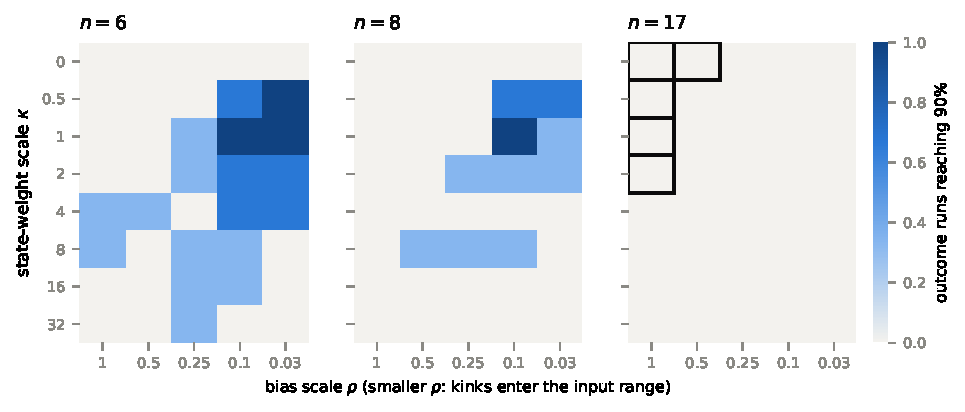
\includegraphics[width=\linewidth]{figures/two_path_sweep.pdf}
\caption{\textbf{Where the outcome trap holds and where it breaks.} Two-path family, zero readout,
three seeds per cell. Cells show the fraction of outcome runs reaching $90\%$ accuracy within $20$k
gradient steps, as the state weights are scaled by $\kappa$ and the biases by $\rho$.
Outlined cells contain seeds that satisfy the outcome certificate. Step training reaches positive
margins in at most $20$ steps in all $360$ runs.}
\label{fig:two-path-sweep}
\end{figure}
